\documentclass[a4paper,10pt,bibliography=totoc]{scrbook}
\usepackage[utf8]{inputenc}
\usepackage[T1]{fontenc}
\usepackage[ngerman]{babel}

%% TYPOGRAPHY
\usepackage{lmodern}  % Latin Modern font
\usepackage{csquotes}

%% GRAPHICS
\usepackage{graphicx}
% Graphics configuration
\DeclareGraphicsExtensions{.pdf,.png}
\graphicspath{{bilder/}}

%% MATH packages
\usepackage{amsmath,amssymb,amsthm}
\usepackage{bbm}
\usepackage{braket}

%% BIBLIOGRAPHY
\usepackage[backend=biber]{biblatex} % biblatex, biber, logreq, etoolbox required
\addbibresource{qm.bib}


\usepackage{hyperref} % hyperref>=6.82a required

% set up PDF information
\hypersetup{
 pdftitle={Grundlagen der Quantenmechanik},
 pdfauthor={Hildegard Uecker, Andreas Sorge},
 pdfsubject={Skript zum Repetitorium},
 hidelinks
}



% Spin (physical quantity)
\newcommand{\Spin}{\ensuremath{\mathbf{S}}} \newcommand{\spin}{\Spin}
\newcommand{\SpinMagnitude}{\ensuremath{S}} \newcommand{\spinm}{\SpinMagnitude}

% magnetic moment (physical quantity)
\newcommand{\MagneticMoment}{\ensuremath{\boldsymbol{\mu}}} \newcommand{\magnmom}{\MagneticMoment}
\newcommand{\MagneticMomentMagnitude}{\ensuremath{\mu}} \newcommand{\magnmomm}{\MagneticMomentMagnitude}

% Bohr magneton
\newcommand{\BohrMagneton}{\ensuremath{\mu_B}} \newcommand{\bohrmag}{\BohrMagneton}

% magnetic field
\newcommand{\MagneticField}{\ensuremath{\mathbf{B}}} \newcommand{\magnf}{\MagneticField}
\newcommand{\MagneticFieldMagnitude}{\ensuremath{B}} \newcommand{\magnfm}{\MagneticFieldMagnitude}
% h-bar / 2
\newcommand{\hbarh}{\ensuremath{\frac{\hbar}{2}}}

% Stern Gerlach apparatus
\newcommand{\SternGerlach}{\ensuremath{\text{SG}}} \newcommand{\sg}{\SternGerlach}

% S_z + state
\newcommand{\SpinZUpState}{\ensuremath{\ket{+}}} \newcommand{\szus}{\SpinZUpState}
% S_z - state
\newcommand{\SpinZDownState}{\ensuremath{\ket{-}}} \newcommand{\szds}{\SpinZDownState}
% S_z +/- state
\newcommand{\SpinZUpDownState}{\ensuremath{\ket{\pm}}} \newcommand{\szs}{\SpinZUpDownState}

% hilbert space
\newcommand{\HilbertSpace}{\ensuremath{\mathcal{H}}} \newcommand{\hs}{\HilbertSpace}

\newcommand{\ComplexNumbers}{\ensuremath{\mathbb{C}}} \newcommand{\comps}{\ComplexNumbers}

% Operator
\newcommand{\Operator}[1]{\ensuremath{\hat{#1}}} \newcommand{\op}[1]{\Operator{#1}}

% S_z operator
\newcommand{\SpinZOperator}{\ensuremath{\op{\SpinMagnitude}_z}} \newcommand{\szop}{\SpinZOperator}

% Dualraum
\newcommand{\DualSpace}[1]{\ensuremath{{#1}^*}} \newcommand{\ds}[1]{\DualSpace{#1}}

% Duale Korrespondenz
\newcommand{\DualCorrespondence}{\ensuremath{\overset{\text{DC}}{\leftrightarrow}}} \newcommand{\dc}{\DualCorrespondence}

% alpha ket
\newcommand{\AlphaKet}{\ensuremath{\ket{\alpha}}} \newcommand{\keta}{\AlphaKet}

% alpha bra
\newcommand{\AlphaBra}{\ensuremath{\bra{\alpha}}} \newcommand{\braa}{\AlphaBra}

% beta ket
\newcommand{\BetaKet}{\ensuremath{\ket{\beta}}} \newcommand{\ketb}{\BetaKet}

% beta bra
\newcommand{\BetaBra}{\ensuremath{\bra{\beta}}} \newcommand{\brab}{\BetaBra}

% complex conjugate
\newcommand{\ComplexConjugate}[1]{\ensuremath{{#1}^*}} \newcommand{\cc}[1]{\ComplexConjugate{#1}}

% X Operator
\newcommand{\OperatorX}{\ensuremath{\op{X}}} \newcommand{\opx}{\OperatorX}
% Y Operator
\newcommand{\OperatorY}{\ensuremath{\op{Y}}} \newcommand{\opy}{\OperatorY}

% AMS Theorem Style Definitions

\theoremstyle{plain}
\newtheorem{erg}{Ergebnis}

\theoremstyle{definition}
\newtheorem{defn}{Definition}
\newtheorem{eig}{Eigenschaft}
\newtheorem{post}{Postulat}
\newtheorem{frage}{Frage}
\newtheorem*{obs}{Beobachtung}
\newtheorem*{zerg}{Zwischenergebnis}
\newtheorem*{zfrage}{Zusatzfrage}

\theoremstyle{remark}
\newtheorem*{antw}{Antwort}
\newtheorem*{bsp}{Beispiel}
\newtheorem*{konv}{Konvention}
\newtheorem*{notiz}{Notiz}


\begin{document}
\pagestyle{headings}

\frontmatter

%% TITLE PAGE
\subject{Skript zum Repetitorium}
\title{Grundlagen der Quantenmechanik}
\author{Hildegard Uecker \and Andreas Sorge}
\publishers{Organisation zur Erforschung komplexer adaptiver Systeme (or-cas)}

\uppertitleback{
\begin{tabbing}
Mathematics and BioSciences Group \quad \= Network Dynamics Group \kill
 \begin{large}Hildegard Uecker\end{large} \> \begin{large}Andreas Sorge\end{large} \\[0.1cm]
 Universit\"at Wien \> MPI f\"ur Dynamik und Selbstorganisation \\
Mathematics and BioSciences Group \> Network Dynamics Group \\
Nordbergstra\ss{}e 15 \> Bunsenstra\ss{}e 10 \\
1090 Wien \> 37073 G\"ottingen \\
\"Osterreich \> Deutschland \\[0.25cm]
\href{mailto:hildegard.uecker@univie.ac.at}{hildegard.uecker@univie.ac.at} \> \href{mailto:as@ds.mpg.de}{as@ds.mpg.de}
\end{tabbing}

\vspace{1cm}
Dieses Skript basiert teilweise auf Vorlagen von Christian K\"ohler, Maria Lenius, Rene Schulz, Christoph Solveen und Fabian Stiewe.

\vspace{1cm}
Dieses Skript wird gepflegt auf GitHub. \\
\url{https://github.com/or-cas/qm-grundlagen}
}

\lowertitleback{Organisation zur Erforschung komplexer adaptiver Systeme (or-cas) e.V.
\vspace{1cm}

\href{http://creativecommons.org/licenses/by-nc-sa/3.0/de/}{
\includegraphics{by-nc-sa-eu}}

Dieses Werk ist unter einer Creative Commons Lizenz vom Typ Namensnennung -- Nicht-kommerziell -- Weitergabe unter gleichen Bedingungen 3.0 Deutschland zugänglich. Um eine Kopie dieser Lizenz einzusehen, konsultieren Sie \url{http://creativecommons.org/licenses/by-nc-sa/3.0/de/} oder wenden Sie sich brieflich an Creative Commons, 444 Castro Street, Suite 900, Mountain View, California, 94041, USA.
}

\maketitle

\chapter*{Vorwort}

Das vorliegende Dokument entsteht als Skript f\"ur eine einw\"ochige Lehrveranstaltung \enquote{Repetitorium Quantenmechanik}  der Verfasser in den Sommersemestern 2011 und 2012 an der Fakult\"at f\"ur Physik der Universit\"at G\"ottingen.

Ziel des Repetitoriums und dieses Skriptes ist, innerhalb von f\"unf Tagen die zentralen theoretischen Inhalte der Pflichtvorlesung \enquote{Quantenmechanik} im Bachelorstudiengang Physik zu wiederholen und anhand von \"Ubungsaufgaben aufzuarbeiten. Unser Schwerpunkt bei Auswahl und Darstellung des Stoffes ist, insbesondere f\"ur die nicht theoretisch oder mathematisch veranlagten Teilnehmer in der gegebenen Zeit einen roten Faden durch Begriffe und vor allem Rechenmethoden der Quantenmechanik zu spinnen. Daf\"ur m\"ussen wir an vielen Stellen auf weiterf\"uhrende Darstellungen verzichten, die \"uber das aus unserer Sicht notwendige Verstehen zum Bestehen hinausgehen, obgleich sie Vorlesungsstoff und damit auch klausurrelevant sein m\"ogen.

Wir danken unseren Vorg\"angern Christian K\"ohler, Maria Lenius, Rene Schulz, Christoph Solveen und Fabian Stiewe f\"ur das Erstellen und \"Uberlassen ihrer Unterlagen f\"ur das Repetitorium Quantenmechanik, die uns wertvolle Anregungen zur Strukturierung und Ausgestaltung unseres Skripts sowie \"Ubungsaufgaben geliefert haben. Die in diesem Skript gemachten Fehler sind nat\"urlich unsere eigenen.

\tableofcontents

\mainmatter

\addchap{Didaktischer Ansatz}

\addchap{Die Woche im \"Uberblick}

\chapter{Montag: Wellenmechanik}

%\usepackage{bbm}
%\usepackage{color}
%\usepackage{caption}
%\usepackage{psfrag}
%\usepackage{esint}
% \parindent0em
% \parskip1.5ex plus0.5ex minus0.5ex
% \topmargin4mm
% \headheight5mm
% \headsep6mm
% \topskip5mm
% \textwidth170mm
% \evensidemargin5mm
% \oddsidemargin5mm
% \textheight210mm
% \hoffset -10mm
% \footskip20mm

%\renewcommand{\textfraction}{0}
%\renewcommand \thesection {\Roman{section}}
%\newcommand{\eps}{\epsilon}
%\newcommand{\qed}{\begin{flushright}$\square$\end{flushright}}

\section{Die Wellenfunktion}

Die Tatsache, da"s Teilchen Welleneigenschaften haben, legt es nahe, 
Teilchen mit Hilfe von Wellen zu beschreiben. Spezielle Wellen sind
die ebenen Wellen:
\begin{equation}
\label{eq::ebene_welle}
	\Psi(\vec x,t) = A e^{i(\vec k \vec x -\omega t)}
\end{equation}
mit einer Dispersionsrelation $\omega = \omega(\vec k)$
(Beispiel Lichtwelle: $\omega = c |\vec k|$).

Ebene Wellen sind "uberall im Raum verteilt. Um ein lokalisiertes Teilchen
zu beschreiben, mu"s man ebene Wellen zu sogenannten Wellenpaketen
"uberlagern:
\begin{equation}
	\Psi(\vec x,t) = \frac{1}{\sqrt{2\pi}}\int \mathrm{d}^3k
	\hat \Psi(\vec k)
	e^{i(\vec k \vec x -\omega t)} = \frac{1}{\sqrt{2\pi}}
	\int \mathrm{d}^3 k\hat \Psi(\vec k,t) e^{(i \vec k \vec x)}.
\end{equation}
Die Funktionen $\Psi$ und $\hat \Psi$ sind also gerade "uber die
Fouriertransformation miteinander verbunden. 

\section{Materiewellen}

F"ur Materiewellen freier Teilchen
gilt mit $E=\hbar \omega$, $\vec p = \hbar \vec k$ und
$E = \frac{|\vec p|^2}{2m}$) die Dispersionsrelation:
\begin{equation}
	\omega(\vec k) = \frac{\hbar |\vec k|^2}{2m}.
\end{equation}
Ableiten der Funktion $\Psi(\vec x,t)$ liefert allgemein:
\begin{align}
	\frac{\partial }{\partial  t} \Psi(\vec x,t) &= 
	\frac{1}{\sqrt{2\pi}}\int \mathrm{d}^3k
        \hat \Psi(\vec k) (-i\omega)
        e^{i(k \vec x -\omega t)}\\
	\Delta \Psi(\vec x,t) &= \frac{1}{\sqrt{2\pi}}\int \mathrm{d}^3k
        \hat \Psi(\vec k) (-|\vec k|^2)
        e^{i(\vec k \vec x -\omega t)}.
\end{align}
Damit gilt f"ur Materiewellen mit obiger Dispersionsrelation:
\begin{equation}
	i\hbar \frac{\partial }{\partial  t} \Psi(\vec x,t)
	= - \frac{\hbar^2}{2m} \Delta \Psi(\vec x,t).
\end{equation}
Die ist die \emph{Schr"odingergleichung f"ur freie Teilchen}.

Was "andert sich f"ur Teilchen in einem Potential $U(\vec x)$?
Es gilt nun $E=\hbar \omega= \frac{\vec p^2}{2m} + U(\vec x)$. Damit
ergibt sich die Schr"odingergleichung:
\begin{equation}
	i\hbar \frac{\partial }{\partial  t} \Psi(\vec x,t)
	= H \Psi(\vec x,t)
\end{equation}
mit dem Hamilton-Operator
\begin{equation}
	H = - \frac{\hbar^2}{2m}\Delta + U(\vec x).
\end{equation}
F"ur L"osungen der Schr"odingergleichung gilt:
\begin{enumerate}
	\item Superpositionsprinzip: Sind $\Psi$, $\phi$ L"osungen,
	dann ist auch $\alpha \Psi + \beta \phi$ mit $\alpha,
	\beta  \in \mathbb{C}$ eine L"osung.
	\item Determiniertheit: Wenn wir $\Psi(\cdot,0)$ kennen, ist
	durch die Schr"odingergleichung die Wellenfunktion zu allen
	Zeiten bestimmt.
	\item Erhaltungssatz: Es gilt $\int \mathrm{d}^3 x
	|\Psi(\vec x,t)|^2 = const.$ (Beweis:
	$\int \mathrm{d}^3 x
        |\Psi(\vec x,t)|^2 = \int \mathrm{d}^3 k
        |\Psi(\vec k,t)|^2 = \int \mathrm{d}^3 k
        |\Psi(\vec k)e^{i\omega t}|^2 = \int \mathrm{d}^3 k
        |\Psi(\vec k)|^2$, wobei wir die Parsevalsche Gleichung verwendet
	haben.)	 
\end{enumerate}

\section{Interpretation der Wellenfunktion als Wahrscheinlichkeitsdichte}

Das Betragsquadrat der normierten Wellenfunktion wird als 
Wahrscheinlichkeitsdichte interpretiert, d.h. $|\Psi(\vec x,t)|^2\mathrm{d}^3x$
gibt die Wahrscheinlichkeit an, das Teilchen zum Zeitpunkt $t$ in einem
Volumenelement $\mathrm{d}^3 t$ am Ort $\vec x$ zu finden. 
Entsprechend ist $|\hat \Psi(\vec k,t)|^2$ die
Wahrscheinlichkeitsdichte f"ur den Wellenvektor (direkter Zusammenhang
zum Impuls: $\vec p = \hbar \vec k$).

Wir betrachten nun die zeitliche Entwicklung der Wahrscheinlichkeitsdichte:
\begin{equation}
\begin{split}
	\frac{\partial }{\partial  t} |\Psi(\vec x,t)\Psi^*(\vec x,t)|^2
	&= \dot \Psi \Psi^* + \Psi \dot \Psi^* =
	-\frac{i}{\hbar} (\hat H\Psi) \Psi^* + \frac{i}{\hbar} 
	\Psi(\hat H\Psi^*)\\
	&= - \frac{i}{\hbar} \left[-\frac{\hbar^2}{2m}(\Delta \Psi)
	+ U(\vec x) \Psi \right] \Psi^* + \frac{i}{\hbar} \Psi
	\left[-\frac{\hbar^2}{2m}(\Delta \Psi^*)+U(\vec x)\Psi^* \right]\\
	&=\frac{\hbar}{2mi} \left[(\Delta \Psi^*)\Psi - (\Delta \Psi)
	\Psi^* \right].
\end{split}
\end{equation}
Mit der Wahrscheinlichkeitsstromdichte $\vec j(\vec x,t) = \frac{\hbar}{2mi}
\left[\Psi^*(\nabla \Psi) - (\nabla \Psi^*)\Psi \right]$ ergibt
sich die Kontinuit"atsgleichung:
\begin{equation}
	\frac{\partial}{\partial t} \rho(\vec x,t) + \nabla \vec j(\vec x,t)=0
\end{equation}
mit
\begin{equation}
	\rho(\vec x,t) = |\Psi(\vec x,t)|^2.
\end{equation}

\section{Quantenmechanische Observablen}

Zun"achst ben"otigen wir einige Definitionen.\\
\textbf{Definition:} Das Skalarprodukt zweier Wellenfunktionen
$\Psi$ und $\phi$ ist gegeben durch
\begin{equation}
	(\phi,\Psi) := \int \mathrm{d}^3 x \phi^*(\vec x)\Psi(\vec x). 
\end{equation}
\textbf{Definition:} $A^{+}$ hei"st zu $A$ adjungierter Operator,
wenn gilt:
\begin{equation}
	(A^+ \phi, \Psi) = (\phi, A \Psi)
\end{equation}
f"ur beliebige $\phi$, $\Psi$.\\
\textbf{Definition:} Der Operator $A$ hei"st hermitisch, wenn $A^+ = A$.
F"ur hermitische Operatoren gilt:
\begin{enumerate}
	\item Eigenwerte hermitischer Operatoren sind reell.
	\item Eigenfunktionen hermitischer Operatoren zu verschiedenen
		Eigenwerten sind orthogonal.
\end{enumerate}
Die Eigenfunktionen der f"ur uns relevanten Operatoren sind vollst"andig,
d.h., sie spannen den ganzen Raum auf.

Observablen werden durch hermitische Operatoren beschrieben. Der Mittelwert
im Zustand $\Psi$ ist gegeben durch
\begin{equation}
	\langle A \rangle = \int \mathrm{d}^3 x \Psi^*(\vec x,t) A \Psi(\vec x,t).
\end{equation}
Die Zeitentwicklung des Mittelwerts wird beschrieben durch:
\begin{equation}
	\frac{\mathrm{d}}{\mathrm{d}t} \langle A \rangle =
	\frac{i}{\hbar} \langle[H,A]\rangle + \langle \frac{\partial A}
	{\partial t}\rangle
\end{equation}
mit dem Kommutator $[B,C] = BC-CB$. Diesen Zusammenhang nennt man
das \emph{Ehrenfestsche Theorem}.

Quantenmechanische Zust"ande $\Psi(\vec x)$ lassen sich nach Eigenfunktionen
hermitischer Operatoren entwickeln, z.B. f"ur ein diskretes Spektrum:
\begin{equation}
	\Psi(\vec x)=\sum \limits_{n} c_n \Psi_n(\vec x) \quad \textnormal{mit}
	\quad c_n = (\Psi_n,\Psi).
\end{equation}
Dabei gilt: $\sum \limits_n |c_n|^2 = 1$. 

F"ur den Mittelwert der Observablen, die durch den Operator $A$ 
beschrieben wird, finden wir:
\begin{equation}
	\langle A \rangle = \sum \limits_{n} |c_n|^2 a_n.
\end{equation}
Interpretation: Mit Wahrscheinlichkeit $|c_n|^2$ messen wir den Wert
$a_n$. Die Wellenfunktion geht dann in den Zustand $\Psi_n$ "uber.

Beispiele f"ur Operatoren (mit kontinuierlichem Spektrum) sind 
der Orts- und der Impulsoperator.\\
\textbf{Ortsoperator (in einer Dimension):} 
\begin{itemize}
	\item Eigenwertgleichung: $x\Psi_{\xi}(x)=\xi \Psi_{\xi}(x)$
	\item Eigenfunktionen: $\Psi_{\xi}(x) = \delta(x-\xi)$.
\end{itemize}
\textbf{Impulsoperator (in einer Dimension):}
\begin{itemize}
	\item Eigenwertgleichung: $\frac{\hbar}{i} \frac{\partial}{\partial x}
		\Psi_p(x) = p \Psi(x)$.
	\item Eigenfunktionen: $\Psi_p(x) = (2 \pi \hbar)^{-1/2}
		e^{ipx/\hbar}$.
\end{itemize}



\section{Die station"are Schr"odingergleichung}

Falls das Potential $U(\vec x)$ zeitunabh"angig ist, kann die 
Schr"odingergleichung mittels eines Separationsansatzes gel"ost werden:
\begin{equation}
	\Psi(\vec x,t) = f(t)\Psi(\vec x).
\end{equation}
Einsetzen dieses Ansatzes leifert: 
\begin{equation}
	\frac{1}{f(t)}i\hbar \frac{\partial}{\partial t} f(t)
	= \frac{1}{\Psi(\vec x)}H\Psi(\vec x).
\end{equation}
Die linke Seite h"angt nur von $t$ ab, die rechte nur von $x$. Beide
Seiten m"ussen also gleich einer Konstanten $E$ sein. Damit ergibt
sich f"ur den zeitabh"angigen Teil:
\begin{equation}
	i\hbar \frac{\partial}{\partial t}f(t)=E f(t)
	\quad \Rightarrow \quad f(t)=e^{-iEt/\hbar}.
\end{equation} 
F"ur den ortsabh"angigen Teil erhalten wir:
\begin{equation}
	H\Psi(\vec x) = E\Psi(\vec x).
\end{equation}
Diese Gleichung nennt man \emph{zeitunabh"angige Schr"odingergleichung}.
(Die Zust"ande $\Psi(\vec x,t) = \exp{(-iEt/\hbar)}\Psi(\vec x)$ 
hei"sen station"are Zust"ande, da gilt: 
$|\Psi(\vec x,t)|^2=|\Psi(\vec x)|^2$.)

Die allgemeine L"osung der Schr"odingergleichung l"a"st sich nun nach
diesen station"aren L"osungen entwickeln:
\begin{equation}
	\Psi(\vec x,t) = \sum \limits_{n} c_n e^{-iE_nt/\hbar}\Psi_n(\vec x)
	\quad \textnormal{mit} \quad c_n = (\Psi_n,\Psi(t=0)).
\end{equation}


\section{Beispiel: Die Potentialstufe}

siehe z.B. Schwabl, Quantenmechanik




\chapter{Dienstag: Dirac-Formalismus}

Wir orientieren uns in diesem Kapitel im Wesentlichen an der Darstellung des \textcite{Sakurai1994Modern} und des \textcite{Nolting2004Grundkurs}.

\section{Der Stern-Gerlach-Versuch}

\emph{Der Stern-Gerlach-Versuch offenbart das Paradigma der Quantenmechanik: Zwei"=Zustands"=Systeme, bei denen die Quantenmechanik unserer liebgewordenen klassischen Intuition und Interpretation am meisten widerspricht!}

\subsection{Aufbau und gemessene Gr\"o\ss{}en}
\begin{figure}
\href{http://commons.wikimedia.org/wiki/File:Stern-Gerlach_Experiment_de.png?uselang=de}{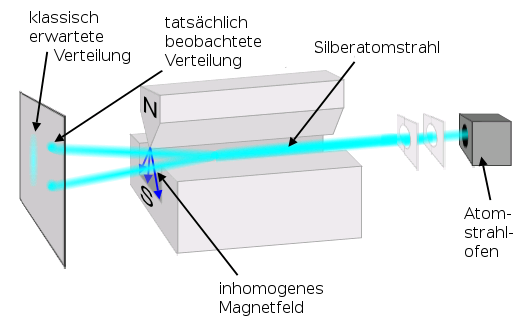
\includegraphics[width=\textwidth]{sterngerlach}}
\caption{\label{fig:SG}Der Stern-Gerlach-Versuch (1922). \href{http://commons.wikimedia.org/wiki/File:Stern-Gerlach_Experiment_de.png?uselang=de}{Grafik: Theresa Knott, Wikimedia Commons}, \href{http://creativecommons.org/licenses/by-sa/3.0/deed.de}{lizenziert unter CreativeCommons-Lizenz by-sa-3.0}.}
\end{figure}

Im in \figurename~\ref{fig:SG} gezeigten und 1922 in Frankfurt a.M.\ durchgef\"uhrten Experiment von Otto Stern und Walther Gerlach werden ungeladene Silberatome in einem Ofen erhitzt. Der aus dem Ofen austretende Strahl ungeladener Silberatome durchl\"auft ein inhomogenes Magnetfeld und trifft auf einen Schirm, auf dem die Intensit\"atsverteilung gemessen wird. Mit der Intensit\"atsverteilung messen wir die Ablenkung der Silberatome im Magnetfeld.

\begin{frage}
 Welche Kraft wirkt auf ein ungeladenes Silberatom in einem inhomogenen Magnetfeld?
\end{frage}
\begin{antw}
Da sie ungeladen sind, wirkt keine Lorentzkraft. Jedes Atom besitzt allerdings ein $5s$-Elektron mit einem Eigendrehimpuls, dem Spin \spin\ mit dem Betrag \hbarh. (Die Drehimpulse der anderen 46 Elektronen heben sich gegenseitig auf.) Daher weist das \emph{Leuchtelektron} und somit das gesamte Atom ein magnetisches Moment \magnmom\ parallel und proportional zum Spin auf: $\magnmom \propto \spin$. Der Betrag des magnetischen Moments des Elektrons (und damit hier des gesamten Atoms) ist das Bohrsche Magneton $\bohrmag = \frac{e}{2m_e}\hbar = |\magnmom|$.
\end{antw}

\begin{frage}
 Wie sieht die Formel der Kraft aus, die auf ein magnetisches Moment \magnmom\ in einem Magnetfeld \magnf\ wirkt?
\end{frage}
\begin{antw}
 Auf ein magnetisches Moment \magnmom\  im (inhomogenen) Magnetfeld \magnf\ wirkt eine Kraft $\mathbf{F} = \nabla (\magnmom \cdot \magnf)$. Wir nehmen an, dass sich das Magnetfeld nur in $z$-Richtung \"andert, sodass $\mathbf{F} = (0,0,F)$ auch nur eine Komponente in $z$-Richtung hat, mit dem Betrag $F= \magnmomm \frac{\partial \magnfm}{\partial z} \cos \alpha$. Hier ist $\alpha = \sphericalangle(\magnmom, \magnf)$ der (konstante) Winkel zwischen magnetischem Moment und Magnetfeld.
\end{antw}

\begin{frage}
 Was misst der Stern-Gerlach-Apparat effektiv?
\end{frage}
\begin{antw}
 Der Stern-Gerlach-Aufbau misst effektiv die Verteilung der Ausrichtungen $\alpha = \sphericalangle(\magnmom, \magnf)$ der magnetischen Momente der Silberatome zum magnetischen Feld. Genauer gesagt misst der Stern-Gerlach-Aufbau die $z$-Komponente $\magnmomm_z$ des magnetischen Moments jedes Silberatoms, und damit die $z$-Komponente $\spinm_z$ des Spins des Leuchtelektrons.
\end{antw}


Die magnetischen Momente \magnmom\ der Silberatome aus dem Ofen sind vor Eintritt in das Magnetfeld zuf\"allig in alle Richtungen orientiert.

\begin{frage}
 Welche qualitative Intensit\"atsverteilung erwarten Sie daher auf dem Schirm?
\end{frage}
\begin{antw}
 Klassisch erwarten wir eine \emph{kontinuierliche} Verteilung zwischen den maximalen Auslenkungen, die gerade der vollst\"andigen Ausrichtung des magnetischen Moments entlang der $z$-Richtung entsprechen ($\magnmomm_z = \pm |\magnmom|$). Wegen der zuf\"alligen Orientierung der magnetischen Momente kommen auch dazwischen alle Werte vor.
\end{antw}

\begin{erg}
 Tats\"achlich beobachten wir im Stern-Gerlach-Experiment, dass der Strahl im Apparat aufgespalten wird und wir zwei \emph{diskrete} Komponenten $z_+$ und $z_-$ erhalten, die gerade den vollst\"andigen Ausrichtungen der magnetischen Momente entsprechen!

Nach der Messung erhalten wir also zwei getrennte Teilstrahlen mit nur den beiden diskreten Werten $\spinm_z = +\hbarh$ and $\spinm_z = -\hbarh$ f\"ur den Spin.
\end{erg}


\begin{zfrage}
 Warum richten sich nicht schon klassisch gesehen alle magnetischen Momente im Magnetfeld aus? 
\end{zfrage}
\begin{antw}
 Magnetische Momente von ruhenden K\"orpern (Stabmagnete z.B.) richten sich in der Tat am Magnetfeld aus. Elektronenspins stehen aber f\"ur eine Eigen\emph{rotation}, und magnetische Momente \magnmom\ rotierender K\"orper behalten ihren Winkel zur Feldrichtung \magnf: sie richten sich nicht aus, sondern pr\"azessieren (wie ein mechanischer Kreisel) unter dem Drehmoment $\magnmom \times \magnf$ um die durch die Feldrichtung \magnf\ gegebene Achse. Dabei bleibt der Winkel zu dieser Achse konstant. W\"urden sich die Elektronenspins tats\"achlich im Magnetfeld ausrichten, m\"ussten zudem alle in Richtung des Magnetfeldes zeigen, und keiner in entgegengesetzte Richtung (wie es aber beim Stern-Gerlach-Experiment beobachtet wird).
\end{antw}

\subsection{Hintereinanderschaltung von Stern-Gerlach-Apparaturen}
\begin{frage}
 Was erwarten Sie (klassisch): Welche Teilstrahlen treten auf, wenn der $z_-$-Teilstrahl aus einem Stern-Gerlach-Apparat $\sg_z$ blockiert wird und nur der $z_+$-Teilstrahl in einen weiteren Stern-Gerlach-Apparat $\sg_z$ geschickt wird?
\end{frage}
\begin{obs}
 Siehe \figurename{}~\ref{fig:seqSQ} oben: Es \"andert sich nichts. Die Spins bleiben in $z_+$-Richtung ausgerichtet.
\end{obs}

\begin{frage}
 Der $z_+$-Teilstrahl aus einer Stern-Gerlach-Apparatur $\sg_z$ wird in einer in $x$-Richtung angeordneten Stern-Gerlach-Apparatur $\sg_x$ wieder zur H\"alfte in zwei Komponenten $x_+$ und $x_-$ aufgeteilt, siehe \figurename{}~\ref{fig:seqSQ} Mitte. Wie erkl\"aren Sie sich dieses Ergebnis?
\end{frage}
Man k\"onnte klassisch vermuten, dass die Spins der Leuchtelektronen der Silberatome im $z_+$-Strahl je zur H\"alfte durch $\spinm_z = +\hbarh, \spinm_x = +\hbarh$ und $\spinm_z = +\hbarh, \spinm_x = -\hbarh$ bestimmt sind.

Aber:
\begin{obs}
Schickt man nur den $x_+$-Teilstrahl aus einer Stern-Gerlach-Apparatur $\sg_x$, der nur aus dem $z_+$-Teilstrahl einer $\sg_z$-Apparatur gewonnen wurde, erneut durch eine $\sg_z$-Apparatur, so spaltet sich dieser erneut je zur H\"alfte in $z_+$ und $z_-$ auf!
\end{obs}

Willkommen in der Quantenmechanik! Denn:
\begin{erg}
 Die Messung von $\spinm_x$ durch die $\sg_x$-Apparatur verbunden mit der Selektion des $x_+$-Zustands vernichtet alle vorherige Information \"uber den Zustand $z_+$. $\spinm_z$ und $\spinm_x$ lassen sich nicht gleichzeitig bestimmen!
\end{erg}

\begin{figure}
 \href{http://commons.wikimedia.org/wiki/File:Sg-seq.svg}{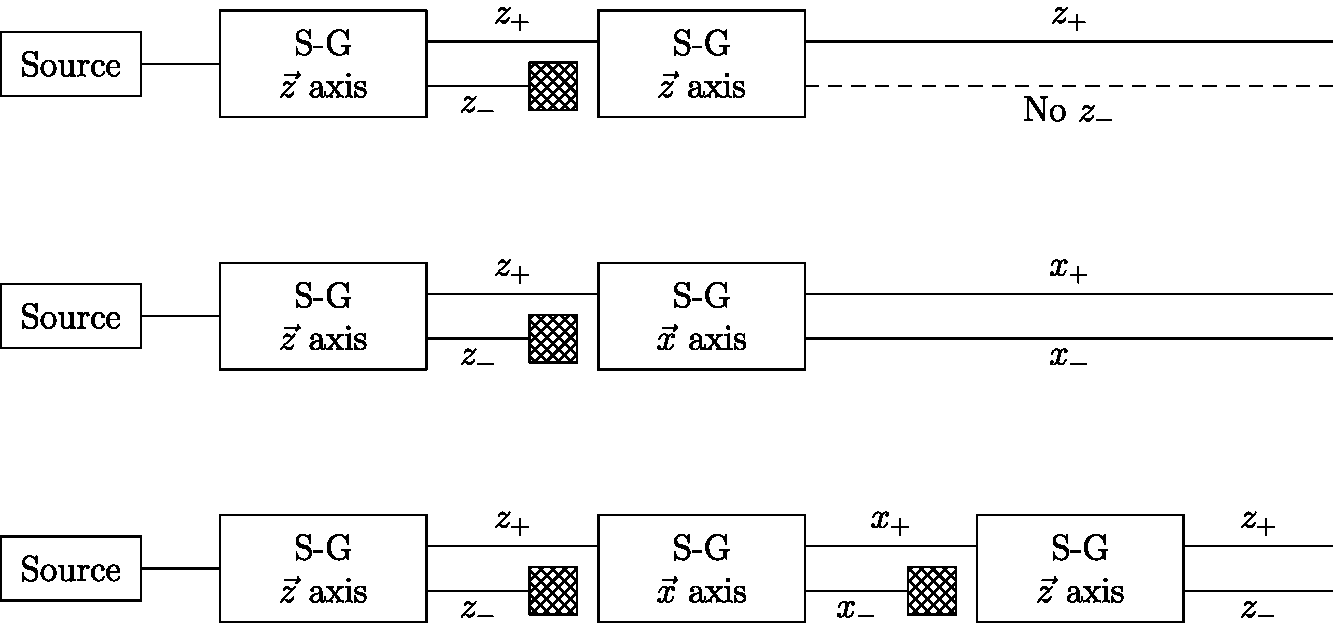
\includegraphics[width=\textwidth]{sequentieller-sterngerlach}}
\caption{\label{fig:seqSQ}Sequentielle Stern-Gerlach-Versuche. \href{http://commons.wikimedia.org/wiki/File:Sg-seq.svg}{Grafik: Francesco Versaci, Wikimedia Commons}, Public Domain.}
\end{figure}


\section{Zust\"ande, Observable, Operatoren}

\section{Physikalische Interpretation}

\section{Das Spin-$\frac{1}{2}$-System und die Pauli-Matrizen}

\section{Die Wellenfunktion im Dirac-Formalismus}

\section{Die Dynamik von Quantensystemen}
\subsection{Zeitentwicklung der Zust\"ande (Schr\"odinger-Bild)}

\subsection{Zeitentwicklung der Observablen (Heisenberg-Bild)}


\chapter{Mittwoch: Harmonischer Oszillator}

% \section{Der harmonische Oszillator}

Der Hamilton-Operator des harmonischen Oszillators ist
\begin{equation}
	\hat H = \frac{\hat  P^2}{2m} + \frac{m\omega^2}{2}\hat X^2.
\end{equation}
Wie wollen nun die station"are Schr"odingergleichung 
\begin{equation}
	\hat H |\Psi\rangle = E|\Psi \rangle
\end{equation}
l"osen. Dazu verwenden wir die Methode der \textbf{Auf- und Absteigeoperatoren}.
(Warum die Operatoren so hei"sen, werden wir weiter unten sehen.)
Der Auf- bzw. Absteigeoperator des harmonischen Oszillators ist gegeben durch
\begin{align}
	\hat a = \frac{\omega m \hat X + i \hat P}{\sqrt{2\omega m \hbar}},
	\hat a^+ = \frac{\omega m \hat X-i\hat P}{\sqrt{2\omega m \hbar}}.
\end{align}
Bemerkung: Die beiden Operatoren sind nicht hermitisch.\\
Damit lassen sich der Orts- und der Impulsoperator schreiben als
\begin{align}
	\hat X = \sqrt{\frac{\hbar}{2\omega m}}(\hat a +\hat a^+),
	\hat P = -i \sqrt{\frac{\hbar \omega m}{2}}(\hat a -\hat a^+).
\end{align}
Es gilt:
\begin{equation}
	[\hat a,\hat a^+] = \hat a \hat a^+ - \hat a^+ \hat a = \mathbbm{\hat 1}.
\end{equation}
Damit lautet der Hamilton-Operator:
\begin{equation}
	\hat H = \frac{1}{2}\hbar \omega (\hat a^+\hat a + \hat a\hat a^+) = \frac{1}{2}\hbar \omega (2\hat a^+\hat a +
	\mathbbm{\hat 1}) = \hbar \omega \left(\hat a^+ \hat a + \frac{1}{2}\right).
\end{equation}
Somit ist das Problem auf die Auffindung der Eigenwerte des \textbf{Besetzungszahloperators}
\begin{equation}
	\hat n = \hat a^+\hat a
\end{equation}
zur"uckgef"uhrt.

Es sei $|\nu\rangle$ Eigenzustand zum Eigenwert $\nu$. Es gilt:
\begin{equation}
\begin{split}
	&\nu \langle \nu|\nu \rangle = \langle \nu|\hat a^+ \hat a|\nu\rangle \geq 0 \quad (=0 \, \textnormal{f"ur} \, |\hat a |\nu\rangle=0). 
	\\
	&\Rightarrow \nu \geq 0.
\end{split}
\end{equation}
D.h. $\nu=0$ ist der niedrigstm"ogliche EW. Gibt es dazu einen EV? Ja! (aus $|\hat a|\nu \rangle =0$ in der Ortsdarstellung
berechenbar). 

Wir werden jetzt die "ubrigen Eigenwerte und Eigenvektoren berechnen. Dazu brauchen wir zun"achst zwei weitere
Relationen:
\begin{align}
	[\hat n, \hat a^+] = \hat a^+,
	[\hat n, \hat a]=-\hat a.
\end{align}
(Denn: $[\underbrace{\hat a^+\hat a}_{\hat n}, \hat a^+] = \hat a^+ \underbrace{[\hat a, \hat a^+]}_{=1} + 
\underbrace{[\hat a^+,\hat a^+]}_{=0} \hat a = \hat a^+$ und 
$[\hat n, \hat a] = \hat a^+ [\hat a, \hat a] + [\hat a^+, \hat a]\hat a=-\hat a$.)

Behauptung: $\hat a^+ |\nu \rangle$ ist Eigenfunktion zum Eigenwert $\nu+1$.
\begin{equation}
	\hat n \hat a^+ |\nu\rangle = (\hat a^+ \hat n + \hat a^+) |\nu\rangle = (\nu+1)\hat a^+ |\nu\rangle.
\end{equation}
Normierung: 
\begin{equation}
	\langle \nu| \hat a \hat a^+|\nu\rangle = \langle \nu|\hat a^+ \hat a + 1|\nu \rangle=
	(\nu+1) \langle \nu|\nu \rangle >0.
\end{equation}
Somit gilt f"ur auf $1$ normierte $|\nu\rangle$, $|\nu+1\rangle$: 
\begin{equation}
	\hat a^+ |\nu\rangle = \sqrt{\nu+1} |\nu+1\rangle.
\end{equation}
Ausgehend von $|0 \rangle$:
\begin{equation}
	 |\nu \rangle = \frac{1}{\sqrt{\nu}}\hat a^+|\nu-1\rangle = \frac{1}{\sqrt{\nu!}}(\hat a^+)^\nu|0\rangle.
\end{equation}
Sind das alle Eigenvektoren?\\
Behauptung: $\hat a |\nu\rangle$ ist Eigenzustand zum Eigenwert $\nu-1$.
\begin{equation}
	 \hat n \hat a |\nu \rangle = (\hat a \hat n -\hat a)|\nu \rangle = (\nu-1)\hat a |\nu\rangle 
\end{equation}
Norm:	 
\begin{equation}
	 \langle \nu|\hat a^+ \hat a| \rangle = \nu \langle \nu |\nu \rangle \, \textnormal{f``ur} 
	 \, \nu\geq 0 \quad (=0 \, \textnormal{f''ur} \, \nu=0).
\end{equation}
F``ur $\nu \geq 1$: $\hat a |\nu \rangle = \sqrt{\nu}|\nu-1\rangle$.\\
Behauptung: Mit $|\nu \rangle$, $\nu=1,2\dots$ sind alle Eigenvektoren gefunden.\\
Beweis durch Widerspruch:\\
Angenommen, es g''abe einen Eigenwert $\nu=n+\alpha$ mit $0<\alpha<1$ und $n \in \mathbbm{N}_0$, d.h.
\begin{equation}
	\hat n|\nu\rangle = (n+\alpha) |\nu\rangle.
\end{equation}
Wegen $\hat a |\nu \rangle = \sqrt{\nu} |\nu-1\rangle$:
\begin{align}
	&\hat n (\hat a^n) |\rangle = \alpha (\hat a^n) |\nu\rangle\\
	&\hat n(\hat a^{n+1})|\nu \rangle = (\alpha-1)(\hat a^{n+1})|\nu \rangle.
\end{align}
$\Rightarrow$ Es g``abe Eigenvektoren von $\hat n$ mit endlicher Norm und negativen Eigenwerten. %$\lightning$ 
Widerspruch: Eigenwerte sind positiv \section{drehimpuls}
\label{sec:drehimpuls}
(s.o.).

F''ur die Energieeigenwerte des harmonischen Oszillators erhalten wir:
\begin{equation}
	E = \hbar \omega \left(n+\frac{1}{2}\right).
\end{equation}
$|0 \rangle$ hei``st Grundzustand, $|\nu \rangle$ hei''st $\nu$-ter angeregter Zustand. 

Die Operatoren $\hat a^+$ bzw. $\hat a$ erh``ohen bzw. erniedrigen den Energieeigenwert um $\hbar \omega$ und
werden deshalb Erzeugungs- und Vernichtungsoperator genannt (auch Leiteroperatoren).

\chapter{Donnerstag: Drehimpuls, Zentralpotential, Wasserstoffatom}

\chapter{Freitag: St\"orungsrechnung}

\addchap{Ausblick}

\backmatter

\printbibliography

\end{document}
